\section{The structure-conduct-performance paradigm}\label{sec:01-scp}

For about three decades the main empirical program in industrial organization put one question to
cross-industry data. Do more concentrated industries earn higher margins? The program is known as the
\emph{structure-conduct-performance} (SCP) paradigm. This section states its logic, formalizes the
experiment it had in mind, and describes how it was carried out. \Cref{sec:01-scp-econometrics} then asks
what its regressions identify, and \cref{sec:01-scp-after} follows the debates it left behind.

\subsection{The SCP mechanism}\label{sec:01-scp-mechanism}

The paradigm describes a causal chain with four links, summarized in \cref{fig:01-scp-flow}. \emph{Basic
conditions} are the primitives of an industry. On the supply side they include technology, unionization,
the transportability of the product and the legal environment. On the demand side they include
preferences, the growth of demand and its seasonality. Basic conditions determine \emph{market
structure}, which comprises the number of sellers and buyers, the extent of vertical integration, and the
degree of vertical and horizontal product differentiation. Structure determines conduct, the
pricing, advertising and investment decisions of firms. Conduct in turn determines \emph{performance},
measured by profits and by welfare.

\citet[Introduction]{Tirole1988} calls this program the ``Harvard tradition'' and associates it with Joe Bain
and Edward Mason. In his history it was the first of two waves of interest in industrial organization, and it
was empirical in nature. His statement of the chain is close to ours. Structure comprises the number of sellers,
their degree of product differentiation, the cost structure and the degree of vertical integration with
suppliers. Conduct comprises price, research and development, investment and advertising. Performance comprises
efficiency, the ratio of price to marginal cost, product variety, the rate of innovation, profits and
distribution. Tirole adds that the paradigm, although plausible, often rested on loose theories.

\begin{figure}[htbp]
\centering
\begin{tikzpicture}[
  box/.style={draw, rounded corners=2pt, align=flush left, text width=3.15cm,
    inner sep=4pt, font=\footnotesize},
  fwd/.style={-{Stealth[length=2.2mm]}, thick},
  back/.style={-{Stealth[length=2mm]}, dashed, gray!65!black},
  lab/.style={font=\scriptsize, align=center, text=gray!25!black}]
\node[box] (bc) {\parbox[t][2.85cm][t]{\linewidth}{\raggedright\textbf{Basic conditions}\\[3pt]
  Supply: technology, unions, transportability, legal environment.\\[3pt]
  Demand: preferences, growth, seasonality.}};
\node[box, right=0.62cm of bc] (ms) {\parbox[t][2.85cm][t]{\linewidth}{\raggedright\textbf{Market structure}\\[3pt]
  Number of sellers and buyers, vertical integration, vertical and horizontal product
  differentiation.}};
\node[box, right=0.62cm of ms] (cd) {\parbox[t][2.85cm][t]{\linewidth}{\raggedright\textbf{Conduct}\\[3pt]
  Pricing, advertising, investment.}};
\node[box, right=0.62cm of cd] (pf) {\parbox[t][2.85cm][t]{\linewidth}{\raggedright\textbf{Performance}\\[3pt]
  Profits, welfare.}};
\draw[fwd] (bc) -- (ms);
\draw[fwd] (ms) -- (cd);
\draw[fwd] (cd) -- (pf);
\draw[back] (cd.-115) to[out=-120, in=-60] node[lab, below=1pt] {mergers, advertising,\\ R\&D}
  (ms.-65);
\draw[back] (pf.-100) to[out=-115, in=-65, looseness=0.85]
  node[lab, below=1pt] {entry and exit respond to profits} (ms.-115);
\draw[back] (cd.110) to[out=125, in=55, looseness=0.8]
  node[lab, above=1pt] {R\&D changes technology, lobbying changes the legal environment}
  (bc.70);
\end{tikzpicture}
\caption{The structure-conduct-performance paradigm. Solid arrows show the causal chain that the
paradigm assumes. Dashed arrows show feedback that it ignores. Conduct and performance shape market
structure, and conduct reshapes basic conditions. Once the dashed arrows are admitted, market structure
is an equilibrium outcome.}
\label{fig:01-scp-flow}
\end{figure}

The chain has a strong implication for policy. If structure causes performance, a regulator can improve
performance by acting on structure, for example by blocking mergers or breaking up dominant firms. The
empirical task then reduces to measuring how performance varies with structure. Conduct rarely needs to
be observed, because structure is assumed to pin it down.

The dashed arrows in \cref{fig:01-scp-flow} show why the chain is incomplete. Profits attract entry and
losses induce exit, so performance feeds back into the number of sellers. Mergers, advertising and
research and development (R\&D) are forms of conduct, yet they shape concentration and differentiation.
Research changes technology and lobbying changes the legal environment, so conduct also feeds back into
basic conditions. In modern terms, market structure is an equilibrium outcome, determined jointly with
conduct and performance by the basic conditions. \Cref{sec:01-scp-econometrics} works out the
consequences of this observation for the regressions that the paradigm relied on.

The ideal experiment behind the paradigm is easy to state. We would take many otherwise identical
industries, randomly assign each one a market structure, and compare their performance. In practice,
researchers compared markups or profitability across existing industries with different levels of
concentration. The gap between the two designs can be stated precisely in the language of potential
outcomes, which \cref{app:econometrics} reviews.

\begin{definition}[Potential margins]\label{def:01-potential-margins}
Index industries by $k = 1, \dots, n$. For each concentration level $h \in (0, 1]$, let $L_k(h)$ be the
industry-wide Lerner index that industry $k$ would have if an outside intervention set its Herfindahl
index to $h$. The intervention holds the demand, costs and conduct of the industry fixed. The function
$h \mapsto L_k(h)$ is the \emph{causal curve} of industry $k$. We observe only the realized margin $L_k
= L_k(\HHI_k)$.
\end{definition}

The industry-wide Lerner index is the share-weighted index $\sum_i s_i L_i$ of
\cref{prop:01-cowling-waterson}. An intervention that sets $h$ could be a regulator that fixes the number
of licenses in an industry of symmetric firms. Now compare the average margins of industries observed at
two concentration levels $h$ and $h'$. We add and subtract $\E[L_k(h') \mid \HHI_k = h]$:
\begin{align}
\E[L_k \mid \HHI_k = h] - \E[L_k \mid \HHI_k = h']
  &= \E[L_k(h) \mid \HHI_k = h] - \E[L_k(h') \mid \HHI_k = h'] \notag \\
  &= \underbrace{\E[L_k(h) - L_k(h') \mid \HHI_k = h]}_{\text{causal effect at } h} \notag \\
  &\quad + \underbrace{\E[L_k(h') \mid \HHI_k = h] - \E[L_k(h') \mid \HHI_k = h']}_{\text{selection}}.
  \label{eq:01-potential-outcomes}
\end{align}
The first equality uses $L_k = L_k(\HHI_k)$. The first term after the second equality is the average
causal effect of moving from $h'$ to $h$ among the industries observed at $h$. The second term compares
the margins that
two different groups of industries would earn at the same concentration $h'$. It differs from zero
whenever the industries that end up concentrated differ in demand, cost or conduct from those that do
not. Random assignment makes $\HHI_k$ independent of the whole curve $L_k(\cdot)$. The selection term
then vanishes, and the first term becomes the population average effect $\E[L_k(h) - L_k(h')]$.

\begin{example}[Selection on the demand elasticity]\label{ex:01-selection-elasticity}
Suppose industry $k$ has constant-elasticity demand with elasticity $\varepsilon_k$ and symmetric
Cournot firms. By \cref{prop:01-cowling-waterson}, its causal curve is
$L_k(h) = \frac{h}{\varepsilon_k}$. Substituting into \eqref{eq:01-potential-outcomes}, the selection
term equals
\[
h' \left( \E\left[\frac{1}{\varepsilon_k} \,\middle|\, \HHI_k = h\right]
        - \E\left[\frac{1}{\varepsilon_k} \,\middle|\, \HHI_k = h'\right] \right).
\]
Its sign depends on how industries sort. Margins are higher where demand is less elastic, so free entry
tends to draw more firms into those industries and to make them less concentrated. The conditional mean
of $\frac{1}{\varepsilon_k}$ then falls with concentration, and the selection term is negative for
$h > h'$. If inelastic demand instead goes with high fixed costs, the term can be positive.
\end{example}

\subsection{Origins and practice}\label{sec:01-scp-practice}

The SCP approach grew out of the Harvard tradition associated with \citet{Mason1939}. As its title indicates,
Mason's article studied the price and production policies of large-scale enterprise.
Joe Bain turned the SCP view into a statistical program. \citet{Bain1951} related
the profit rates of American manufacturing industries over 1936--1940 to their concentration.
\citet{Bain1951,Bain1956} hypothesized that concentration facilitates collusion between firms and so raises
industry-wide profits \citep[Section~5.5]{Tirole1988}. \citet[p.~46]{LevensteinSuslow2006} attribute the same
hypothesis to Bain. \citet{Bain1956} added the theory of \emph{barriers to entry}, the advantages of established
sellers over potential entrants. In Tirole's paraphrase, a barrier to entry is anything that lets incumbent firms
earn supranormal profits without the threat of entry \citep[Chapter~8, introduction]{Tirole1988}. Tirole lists
the four elements of market structure that Bain identified informally. They are economies of scale, absolute cost
advantages, product-differentiation advantages and capital requirements, the last of which Tirole calls
controversial. Bain also distinguished three cases. Entry is blockaded when incumbents ignore the threat and entry
is still unattractive. It is deterred when incumbents change their behavior to prevent it, and accommodated when
they find it more profitable to let entrants in. For the quarter century that followed \citet{Bain1951}, the
cross-section study of many industries was the main empirical method of the field \citep[p.~1012]{Bresnahan1989}.
\citet{Schmalensee1989} wrote its definitive review.

A typical study used one cross-section of industries. The dependent variable was an accounting measure
of profitability, such as the profit rate on equity or assets or the price-cost margin computed from the
Census of Manufactures. The key regressor was a concentration measure, often the four-firm ratio
$\mathit{CR}_4$ or the Herfindahl index of \cref{def:01-concentration}. The canonical specification is
\begin{equation}\label{eq:01-scp-regression}
\pi_k = \beta_0 + \beta_1 \HHI_k + \varphi^\top X_k + e_k, \qquad k = 1, \dots, n,
\end{equation}
where $\pi_k$ is the profitability measure of industry $k$ and $e_k$ is an error term. The Herfindahl
index may be replaced by $\mathit{CR}_{4,k}$. The vector $X_k$ collects controls, typically the ratios of
R\&D spending, capital and advertising spending to sales, together with the import share. Its
coefficients are $\varphi$, and the whole equation is estimated by ordinary least squares (OLS). The typical finding was
$\hat\beta_1 > 0$. It was read as evidence that concentration raises margins, and hence that
concentration is harmful.

\citet[Introduction]{Tirole1988} writes the typical regression as $\pi_k = f(\mathit{CR}_k, \mathit{BE}_k, \dots)$,
run on a cross-section of many industries. Here $\mathit{CR}_k$ is a concentration ratio and $\mathit{BE}_k$
collects measures of barriers to entry. Two common measures were the ratio of advertising to sales and the
\emph{minimum efficient scale} of entry, the smallest output at which average cost reaches its minimum.
Regression \eqref{eq:01-scp-regression} is the linear version. Tirole stresses that its coefficients are
correlations, or ``descriptive statistics,'' and not causal relationships. Industry profit, the concentration
ratio and the ratio of advertising to sales ``are jointly endogenous.'' The basic conditions of the market and
the behavior of its firms determine all three at once.

The tradition also tried to measure basic conditions directly, scale economies in particular
\citep[Introduction, note~4]{Tirole1988}. The most common method estimates a cost function of output and input
prices. Bain built ``engineering production functions'' from engineering data on plants, and he asked managers
what the optimal plant size was. George Stigler's \emph{survivorship technique} infers efficient scale instead
from the sizes of the firms that survive. Tirole notes that such measures are hard to make accurate and
comparable across industries.

The design reflected the econometric practice of its time. Samples were small, the data were industry
aggregates, and matrices were sometimes inverted by hand. Identification in the modern sense received
little attention. Concentration was treated as an exogenous regressor, and its coefficient was read as a
structural constant.

\citet[p.~146]{EinavLevin2010} describe two challenges that held the field back into the 1970s. The
first was the lack of compelling theoretical models of imperfect competition, which the game theory
revolution of the 1980s later supplied. The second was the lack of good data and of convincing
strategies for testing hypotheses about competition. Researchers knew that concentration might depend on
the same factors as profitability. More sophisticated studies tried to fix this by treating concentration
as driven by ``exogenous'' barriers to entry, such as scale economies, advertising or R\&D
\citep[p.~146]{EinavLevin2010}. Yet advertising intensity and capital intensity are chosen by firms, so
they are hard to defend as instruments \citep[p.~147]{EinavLevin2010}. \citet[p.~954]{Schmalensee1989}
opened his review by acknowledging that ``essentially all variables that have been employed in such
studies are logically endogenous'' (quoted in \citealp[p.~147]{EinavLevin2010}).

\citet[Introduction, note~2]{Tirole1988} recommends the review of \citet{Schmalensee1989}, which he dates 1986,
as an excellent survey and assessment of this approach. His own summary of the evidence records two facts that frame the rest
of this chapter (note~3). First, the cross-industry relation between rates of return and concentration ``is weak.'' Second,
``introducing a market-share variable on the right-hand side of the regression tends to wipe out
concentration-ratio effects.'' Tirole explains the second fact by cost heterogeneity. In industries where a few
low-cost firms produce most of the output, concentration and profits are both high. The concentration ratio may
then pick up the effect of the omitted market share. The first fact motivates \cref{sec:01-scp-econometrics},
and the second lies at the center of the Demsetz debate in \cref{sec:01-demsetz}. \Cref{sec:01-neio-principles} returns to the maintained
hypotheses of the paradigm that the next generation of research rejected.

\section{What cross-industry regressions identify}\label{sec:01-scp-econometrics}

Regression \eqref{eq:01-scp-regression} always estimates something. Its probability limit is a
linear projection coefficient, and the question is whether that coefficient measures an economic
object. This section takes the problems in turn. Margins are mismeasured (\cref{sec:01-accounting}),
concentration is mismeasured (\cref{sec:01-market-def-error}), and concentration is endogenous
(\cref{sec:01-endogeneity}). A Monte Carlo experiment shows the size of the problems
(\cref{sec:01-montecarlo}), and \cref{sec:01-salinger} asks whether panel data solve them.

\subsection{Measurement: accounting versus economic margins}\label{sec:01-accounting}

The theory of \cref{sec:01-cournot-hhi} concerns the Lerner index $L = \frac{p - mc}{p}$. SCP studies
used accounting data instead. The most common margin was the \emph{Census price-cost margin},
\begin{equation}\label{eq:01-pcm}
\mathit{PCM} = \frac{\text{value of shipments} - \text{payroll} - \text{cost of materials}}
                    {\text{value of shipments}},
\end{equation}
computed for each manufacturing industry from the Census of Manufactures. It nets out the main variable
inputs and ignores the cost of capital. The next proposition shows what it measures. In this subsection
only, $\rho$ denotes the rental price of capital (elsewhere in the book $\rho$ is the pass-through rate).

\begin{proposition}[What the Census margin measures]\label{prop:01-pcm-bias}
Consider an industry that sells output $q > 0$ at price $p$, so that sales are $S = pq$. Payroll and
materials form the variable cost $VC(q)$, with $VC(0) = 0$ and marginal cost $mc(q) = VC'(q)$. The
industry uses a capital stock $K$ with rental price $\rho$, the interest and depreciation cost per dollar
of capital. Economic profit is $\pi = pq - VC(q) - \rho K$.
\begin{enumerate}[label=(\roman*)]
\item If $VC(q) = cq$, then $\mathit{PCM} = \frac{p - c}{p} = L$.
\item In general, $\mathit{PCM} = \frac{\pi}{S} + \rho \frac{K}{S}$. An industry that earns zero economic
profit has $\mathit{PCM} = \rho \frac{K}{S} > 0$.
\item If $VC$ is convex, then $\mathit{PCM} \ge L$. The inequality is strict if $VC$ is strictly convex.
\end{enumerate}
\end{proposition}

\begin{proof}
By definition, $\mathit{PCM} = \frac{S - VC(q)}{S}$. For (i), substitute $VC(q) = cq$:
\[
\mathit{PCM} = \frac{pq - cq}{pq} = \frac{p - c}{p} = L.
\]
For (ii), the definition of economic profit gives $pq - VC(q) = \pi + \rho K$. Divide both sides by $S$:
\[
\mathit{PCM} = \frac{pq - VC(q)}{S} = \frac{\pi + \rho K}{S} = \frac{\pi}{S} + \rho \frac{K}{S}.
\]
Setting $\pi = 0$ gives $\mathit{PCM} = \rho \frac{K}{S}$, which is positive whenever $K > 0$. For (iii),
write $\mathit{PCM} = \frac{p - AVC(q)}{p}$ with average variable cost $AVC(q) = \frac{VC(q)}{q}$. A convex
function lies above its tangent lines, so
\[
VC(0) \ge VC(q) + VC'(q)(0 - q).
\]
With $VC(0) = 0$, this reads $q \, mc(q) \ge VC(q)$, so $AVC(q) \le mc(q)$. Therefore
\[
\mathit{PCM} = \frac{p - AVC(q)}{p} \ge \frac{p - mc(q)}{p} = L.
\]
Strict convexity makes the tangent inequality strict for $q > 0$.
\end{proof}

The Census margin therefore mixes three things: the Lerner index, the return to capital, and the
curvature of variable cost. Capital-intensive industries show high margins even when they earn no rents.
Capital intensity also tends to raise minimum efficient scale and hence concentration. A regression of
$\mathit{PCM}$ on concentration that omits capital intensity then attributes the return to capital to
concentration.

\begin{corollary}[Omitted capital intensity]\label{prop:01-pcm-ovb}
Suppose economic profitability satisfies $\frac{\pi_k}{S_k} = \beta_0 + \beta_1 \HHI_k + e_k$, where
$e_k$ is uncorrelated with $\HHI_k$ and with $\frac{K_k}{S_k}$, and the rental price $\rho$ is common to
all industries. Then OLS of $\mathit{PCM}_k$ on a constant and $\HHI_k$ converges to
\[
\beta_1 + \rho \, \frac{\Cov\left(\frac{K_k}{S_k}, \HHI_k\right)}{\Var(\HHI_k)}.
\]
\end{corollary}

\begin{proof}
By \cref{prop:01-pcm-bias}(ii), $\mathit{PCM}_k = \beta_0 + \beta_1 \HHI_k + \rho \frac{K_k}{S_k} + e_k$.
The OLS slope converges to $\frac{\Cov(\mathit{PCM}_k, \HHI_k)}{\Var(\HHI_k)}$. Substituting,
\[
\frac{\Cov(\mathit{PCM}_k, \HHI_k)}{\Var(\HHI_k)}
 = \beta_1 + \rho \frac{\Cov\left(\frac{K_k}{S_k}, \HHI_k\right)}{\Var(\HHI_k)}
   + \frac{\Cov(e_k, \HHI_k)}{\Var(\HHI_k)},
\]
and the last term is zero by assumption.
\end{proof}

This is why \citet{CollinsPreston1969} and most later studies included the capital-sales ratio
$\frac{K}{S}$ as a regressor next to concentration. The control removes the bias in
\cref{prop:01-pcm-ovb} only if $\rho$ is common across industries and capital is measured correctly.

Accounting rates of return on equity or assets have their own problems. \citet{FisherMcGowan1983} showed
that the accounting rate of return can differ widely from the economic rate of return, which is the
internal rate of return on an investment. The gap depends on the time profile of cash flows and on
depreciation rules, so it varies across industries even when no industry earns rents. Inflation and the
valuation of assets at historical cost add further distortions. A simple case shows the direction of
one common bias.

\begin{remark}[Expensed intangible capital]\label{rem:01-intangibles}
Consider a firm in a steady state with tangible capital $K$. It also builds an intangible stock $A$, such
as brand capital or knowledge, by spending $I$ per period on advertising or R\&D. The stock depreciates
at rate $d_A$, so in the steady state $A = \frac{I}{d_A}$. Let $R$ be revenue net of variable costs and
of the depreciation of tangible capital. Economic depreciation of the intangible stock is $d_A A = I$, so
the economic rate of return on all capital is
\[
r^e = \frac{R - d_A A}{K + A} = \frac{R - I}{K + A}.
\]
Accounting rules expense $I$ and leave $A$ off the balance sheet, so the accounting rate of return is
$r^{acc} = \frac{R - I}{K}$. Dividing the two expressions gives
\[
\frac{r^{acc}}{r^e} = \frac{K + A}{K} = 1 + \frac{A}{K} > 1.
\]
When $R > I$, accounting returns overstate economic returns, and they do so most in industries that are
intensive in advertising or R\&D. If those industries are also more concentrated, the measured profit-concentration relation is
biased upward.
\end{remark}

The controls that theory calls for are the demand elasticity, the height of entry barriers and the degree
of product differentiation. They are hard to measure, so SCP studies rarely included them. The
regression thus omits the very variables that theory says determine margins. \Cref{sec:01-cournot-hhi}
showed that the slope of margins on concentration is $\frac{1 - \kappa}{\varepsilon}$, which depends on
conduct and on the demand elasticity. \Cref{tab:01-scp-data} compares what theory needs with what the
studies measured.

\begin{table}[htbp]
\centering\footnotesize
\renewcommand{\arraystretch}{1.2}
\caption{What the theory of margins needs and what SCP studies measured}
\label{tab:01-scp-data}
\begin{tabularx}{\linewidth}{@{}>{\raggedright\arraybackslash}p{2.1cm}
  >{\raggedright\arraybackslash}X>{\raggedright\arraybackslash}X>{\raggedright\arraybackslash}X@{}}
\toprule
Object & What theory needs & What SCP studies used & Consequence for the regression \\
\midrule
Margin & Lerner index $\frac{p - mc}{p}$ & Accounting profit rate, return on assets, Census
  $\mathit{PCM}$ & Mixes rents with the return to capital and cost curvature
  (\cref{prop:01-pcm-bias}, \cref{rem:01-intangibles}) \\
Concentration & Shares in the economic market (\cref{sec:01-market-definition}) & National shares in a
  four-digit SIC industry & Measurement error and attenuation (\cref{sec:01-market-def-error}) \\
Demand elasticity & $\varepsilon$, which scales the slope & Rarely measured & Omitted variable that
  enters the slope itself \\
Entry barriers & Sunk and fixed costs, regulation & Capital, advertising and R\&D intensities &
  The proxies are chosen by firms, hence endogenous \\
Differentiation & Substitution patterns among products & Advertising intensity, at best & Crude and
  endogenous proxy \\
Conduct & $\kappa$ or $\theta$ (\cref{prop:01-clarke-davies}) & Not measured, implicitly common & The
  slope averages over conduct regimes (\cref{prop:01-scp-plim}) \\
Foreign competition & Imports in the relevant market & Import share & Partial correction of national
  shares \\
\bottomrule
\end{tabularx}
\end{table}

\subsection{Market definition and measurement error in concentration}\label{sec:01-market-def-error}

Concentration is defined relative to a market (\cref{sec:01-market-definition}). SCP studies used
industries as defined by the Standard Industrial Classification (SIC), usually at the four-digit level.
The SIC was replaced by the North American Industry Classification System (NAICS) in 1997. These
classifications group plants by production process more than by substitution in demand. A four-digit
industry can be too broad, pooling products that do not compete with each other. It can also be too
narrow, leaving out close substitutes classified elsewhere and leaving out imports. Census concentration
ratios are national, while many products are sold in local markets because transport is costly. Cement,
ready-mixed concrete and newspapers are standard examples. The next lemma shows how large the resulting
error can be.

\begin{lemma}[Pooling local markets]\label{prop:01-pooled-hhi}
Suppose a national industry consists of $G$ local markets of equal size. Each local market $\ell$ is
served by its own firms and has Herfindahl index $\HHI_\ell$. Then the national Herfindahl index is
\[
\HHI^{nat} = \frac{1}{G} \left( \frac{1}{G} \sum_{\ell = 1}^{G} \HHI_\ell \right).
\]
\end{lemma}

\begin{proof}
Let $s_{i\ell}$ be the share of firm $i$ in local market $\ell$. Because the markets have equal size, the
national share of that firm is $\frac{s_{i\ell}}{G}$. Summing squared national shares over all firms,
\[
\HHI^{nat} = \sum_{\ell = 1}^{G} \sum_{i} \left( \frac{s_{i\ell}}{G} \right)^2
 = \frac{1}{G^2} \sum_{\ell = 1}^{G} \sum_{i} s_{i\ell}^2
 = \frac{1}{G^2} \sum_{\ell = 1}^{G} \HHI_\ell .
\]
Rearranging the last expression gives the result.
\end{proof}

National concentration thus understates local concentration by the factor $G$. Two industries with the
same local Herfindahl index of $0.5$, one sold nationally and one sold in 50 separate local markets, have
national indices of $0.5$ and $0.01$. The number of local markets differs across industries with transport
costs, so this error is large, systematic and correlated with industry characteristics. It cannot be
treated as noise.

Even classical noise has a known cost. Suppose the true relation is $L_k = \beta_0 + \beta_1 \HHI^*_k +
e_k$, and we observe $\HHI_k = \HHI^*_k + u_k$. Assume $u_k$ has mean zero and variance $\sigma_u^2$ and
is uncorrelated with $\HHI^*_k$ and $e_k$. The OLS slope of $L_k$ on $\HHI_k$ converges to
\begin{equation}\label{eq:01-attenuation}
\frac{\Cov(\beta_0 + \beta_1 \HHI^*_k + e_k, \, \HHI^*_k + u_k)}{\Var(\HHI^*_k + u_k)}
 = \frac{\beta_1 \Var(\HHI^*_k)}{\Var(\HHI^*_k) + \sigma_u^2}
 \equiv \beta_1 \chi .
\end{equation}
The numerator keeps only $\beta_1 \Var(\HHI^*_k)$ because the other covariances are zero. The
\emph{reliability ratio} $\chi \in (0, 1]$ is the share of the variance of measured concentration that
is signal. Measurement error biases the slope toward zero, and \cref{sec:01-salinger} shows that panel
methods can make this bias much worse.

\subsection{Endogeneity of structure: theory}\label{sec:01-endogeneity}

Suppose margins and concentration were measured without error. OLS still converges to a projection
coefficient, and the next proposition characterizes it. The industry-level model is the
conduct-adjusted Cowling-Waterson relation of \cref{prop:01-clarke-davies}
\citep{CowlingWaterson1976,ClarkeDavies1982}.

\begin{proposition}[What the SCP slope converges to]\label{prop:01-scp-plim}
Let $(L_k, \HHI_k)$ be independent and identically distributed across industries with finite second
moments and $\Var(\HHI_k) > 0$.
\begin{enumerate}[label=(\roman*)]
\item The OLS slope of $L_k$ on a constant and $\HHI_k$ converges in probability to
$\frac{\Cov(L_k, \HHI_k)}{\Var(\HHI_k)}$.
\item Suppose every industry satisfies $L_k = A_k + B_k \HHI_k$ with $A_k = \frac{\kappa_k}{\varepsilon_k}$
and $B_k = \frac{1 - \kappa_k}{\varepsilon_k}$, where $\kappa_k$ is the Clarke-Davies conduct parameter and
$\varepsilon_k$ the market elasticity of industry $k$. Then the slope converges to
\begin{equation}\label{eq:01-scp-plim}
\E[B_k] + \frac{\Cov(A_k, \HHI_k) + \Cov(B_k, \HHI_k^2) - \E[\HHI_k] \Cov(B_k, \HHI_k)}{\Var(\HHI_k)}.
\end{equation}
\item If $(\kappa_k, \varepsilon_k)$ is independent of $\HHI_k$, the slope converges to
$\E\left[\frac{1 - \kappa_k}{\varepsilon_k}\right]$ and the intercept to
$\E\left[\frac{\kappa_k}{\varepsilon_k}\right]$.
\end{enumerate}
\end{proposition}

\begin{proof}
(i) The OLS slope is the ratio of the sample covariance of $(L_k, \HHI_k)$ to the sample variance of
$\HHI_k$. By the law of large numbers each converges to its population counterpart, and the continuous
mapping theorem gives the limit of the ratio. (ii) Write $H = \HHI_k$ and drop the index $k$. Then
$\Cov(L, H) = \Cov(A, H) + \Cov(BH, H)$. Expand the second term:
\[
\Cov(BH, H) = \E[BH^2] - \E[BH]\,\E[H].
\]
Use $\E[BH^2] = \E[B]\,\E[H^2] + \Cov(B, H^2)$ and $\E[BH] = \E[B]\,\E[H] + \Cov(B, H)$:
\begin{align*}
\Cov(BH, H) &= \E[B]\,\E[H^2] + \Cov(B, H^2) - \E[B]\,\E[H]^2 - \E[H] \Cov(B, H) \\
            &= \E[B] \Var(H) + \Cov(B, H^2) - \E[H] \Cov(B, H).
\end{align*}
Add $\Cov(A, H)$ and divide by $\Var(H)$ to obtain \eqref{eq:01-scp-plim}. (iii) Independence sets
$\Cov(A, H)$, $\Cov(B, H)$ and $\Cov(B, H^2)$ to zero, so the slope converges to $\E[B]$. The intercept
converges to
\[
\E[L] - \E[B]\,\E[H] = \E[A] + \E[BH] - \E[B]\,\E[H] = \E[A] + \Cov(B, H) = \E[A].
\qedhere
\]
\end{proof}

Part (iii) is the best case, the analogue of random assignment in \eqref{eq:01-potential-outcomes}. Even
then the slope is an average of $\frac{1 - \kappa_k}{\varepsilon_k}$ that mixes conduct with the demand
elasticity. It predicts the effect of a policy that changes concentration only if the policy leaves
conduct and elasticities unchanged. Part (ii) shows how sorting moves the slope. Sorting on conduct moves
both terms, because a higher $\kappa_k$ raises $A_k$ and lowers $B_k$. With a common elasticity
$\varepsilon$, $B_k = \frac{1}{\varepsilon} - A_k$, and the bias term in \eqref{eq:01-scp-plim} becomes
\[
\frac{\Cov\left(A_k, g(\HHI_k)\right)}{\Var(\HHI_k)}, \qquad g(h) = (1 + \E[\HHI_k])\,h - h^2 .
\]
The function $g$ increases for $h < \frac{1 + \E[\HHI_k]}{2}$, a range that contains most observed values of
the index. Suppose collusive industries are less concentrated, in the sense that $\E[A_k \mid \HHI_k]$ falls
with $\HHI_k$, and every $\HHI_k$ lies where $g$ increases. Then the covariance is negative, because a
decreasing and an increasing function of the same variable covary negatively. The slope is then biased down,
and Exercise~3 in \cref{sec:01-exercises} gives a case in which it falls to zero. The weaker condition
$\Cov(A_k, \HHI_k) < 0$ does not fix the sign. When $(\kappa_k, \varepsilon_k)$ and $\HHI_k$ are jointly
determined, as they are under free entry, the slope has no structural meaning. The following model makes this
concrete.

\casehead{Free entry with Cournot competition}Each industry has inverse demand $P = a - bQ$ with
$a > c > 0$ and $b > 0$. Firms have constant marginal cost $c$ and pay a fixed cost $F > 0$ to enter.
In stage one, potential entrants decide whether to enter.
In stage two, the $N$ entrants play the symmetric Cournot game, whose equilibrium has
$P - c = \frac{a - c}{N + 1}$ and $q = \frac{a - c}{b(N + 1)}$ (\cref{sec:01-cournot-hhi}). We treat $N$
as continuous, as in the full worked problem of \cref{app:problems}. The free-entry equilibrium follows in
four steps. Profit per firm is
\begin{equation}\label{eq:01-fe-profit}
\pi(N) = (P - c) q - F = \frac{(a - c)^2}{b (N + 1)^2} - F.
\end{equation}
Zero profit, $\pi(N^*) = 0$, gives
\begin{equation}\label{eq:01-fe-N}
N^* + 1 = \frac{a - c}{\sqrt{bF}}, \qquad N^* = \frac{a - c}{\sqrt{bF}} - 1.
\end{equation}
The free-entry dollar markup is therefore
\begin{equation}\label{eq:01-fe-markup}
m^* \equiv P^* - c = \frac{a - c}{N^* + 1} = \sqrt{bF}.
\end{equation}
Concentration and the Lerner index follow:
\begin{equation}\label{eq:01-fe-HL}
\HHI^* = \frac{1}{N^*} = \frac{1}{\frac{a - c}{m^*} - 1} = \frac{m^*}{a - c - m^*}, \qquad
L^* = \frac{P^* - c}{P^*} = \frac{m^*}{c + m^*}.
\end{equation}
The equilibrium has at least one firm when $N^* \ge 1$, that is, when $m^* \le \frac{a - c}{2}$, or
$F \le \frac{(a - c)^2}{4b}$. Every free-entry industry lies on its own Cournot causal curve. With
$bQ^* = N^* m^*$, the elasticity is $\varepsilon^* = \frac{P^*}{bQ^*} = \frac{c + m^*}{N^* m^*}$ and
\[
\frac{\HHI^*}{\varepsilon^*} = \frac{1}{N^*} \cdot \frac{N^* m^*}{c + m^*} = \frac{m^*}{c + m^*} = L^*.
\]
Free entry selects the point on the curve, and the same primitives also shift the curve.

The comparative statics follow from \eqref{eq:01-fe-HL}. Both outcomes rise with $m^*$:
\[
\frac{\partial \HHI^*}{\partial m^*} = \frac{a - c}{(a - c - m^*)^2} > 0, \qquad
\frac{\partial L^*}{\partial m^*} = \frac{c}{(c + m^*)^2} > 0 .
\]
Because $m^* = \sqrt{bF}$, a higher fixed cost or a higher slope $b$ raises both. The slope $b$ measures
market size inversely, since doubling the number of consumers at every price halves $b$. The demand
intercept enters only $\HHI^*$:
\[
\frac{\partial \HHI^*}{\partial a} = -\frac{m^*}{(a - c - m^*)^2} < 0, \qquad
\frac{\partial L^*}{\partial a} = 0 .
\]
Marginal cost moves the two outcomes in opposite directions:
\[
\frac{\partial \HHI^*}{\partial c} = \frac{m^*}{(a - c - m^*)^2} > 0, \qquad
\frac{\partial L^*}{\partial c} = -\frac{m^*}{(c + m^*)^2} < 0 .
\]
Across industries, margins and concentration are therefore positively correlated if fixed costs or
market size vary. They are uncorrelated if only the level of demand varies, and negatively correlated if
only marginal cost varies.

\casehead{Collusion with free entry}Suppose instead that the firms in an industry collude perfectly,
charge the monopoly price and split output equally. \Cref{ch:collusion-theory} studies when such
collusion can be sustained. The joint monopoly solution has $Q^m = \frac{a - c}{2b}$ and $P^m = \frac{a + c}{2}$, so each of $N$ firms earns
\[
\frac{(P^m - c) Q^m}{N} - F = \frac{(a - c)^2}{4bN} - F.
\]
Zero profit gives the number of collusive firms and the two outcomes:
\begin{equation}\label{eq:01-collusion-fe}
N^m = \frac{(a - c)^2}{4bF}, \qquad L^m = \frac{a - c}{a + c}, \qquad
\HHI^m = \frac{1}{N^m} = \frac{4bF}{(a - c)^2}.
\end{equation}
Total fixed costs $N^m F = \frac{(a - c)^2}{4b}$ equal the monopoly profit, so entry dissipates the whole
rent while consumers still pay the monopoly price. Now let $x = \frac{a - c}{\sqrt{bF}} \ge 2$, so
$N^* = x - 1$ and $N^m = \frac{x^2}{4}$. Then
\[
N^m - N^* = \frac{x^2}{4} - x + 1 = \left( \frac{x}{2} - 1 \right)^2 \ge 0 .
\]
The collusive industry also has the higher margin, because $P^* = c + \sqrt{bF} \le c + \frac{a - c}{2}
= P^m$ whenever $x \ge 2$. Collusion raises margins, attracts entry and lowers concentration.

Under collusion, $F$ and $b$ move only $\HHI^m$. The demand intercept and marginal cost move the margin
according to
\[
\frac{\partial L^m}{\partial a} = \frac{2c}{(a + c)^2} > 0, \qquad
\frac{\partial L^m}{\partial c} = -\frac{2a}{(a + c)^2} < 0 ,
\]
while $\HHI^m$ falls with $a$ and rises with $c$. Both primitives therefore move $L^m$ and $\HHI^m$ in
opposite directions. \Cref{tab:01-free-entry-cs} collects the signs.

\begin{table}[htbp]
\centering\small
\caption{Comparative statics of concentration and margins under free entry}
\label{tab:01-free-entry-cs}
\begin{threeparttable}
\begin{tabular}{lcccccc}
\toprule
 & \multicolumn{3}{c}{Cournot} & \multicolumn{3}{c}{Collusion} \\
\cmidrule(lr){2-4}\cmidrule(lr){5-7}
Primitive that rises & $\HHI^*$ & $L^*$ & Co-movement & $\HHI^m$ & $L^m$ & Co-movement \\
\midrule
Demand intercept $a$ & $-$ & $0$ & None & $-$ & $+$ & Negative \\
Marginal cost $c$ & $+$ & $-$ & Negative & $+$ & $-$ & Negative \\
Demand slope $b$ (smaller market) & $+$ & $+$ & Positive & $+$ & $0$ & None \\
Fixed cost $F$ & $+$ & $+$ & Positive & $+$ & $0$ & None \\
\bottomrule
\end{tabular}
\begin{tablenotes}\footnotesize
\item Notes: Linear inverse demand $P = a - bQ$, constant marginal cost $c$, fixed cost $F$, continuous
number of firms. Cournot values from \eqref{eq:01-fe-HL}, collusion values from \eqref{eq:01-collusion-fe}.
``Co-movement'' is the sign of the relation between $L$ and $\HHI$ traced out when only that primitive
varies across industries.
\end{tablenotes}
\end{threeparttable}
\end{table}

\casehead{Mixing conduct}Compare two industries with identical primitives, one Cournot and one
collusive. The collusive industry has the higher margin and, under free entry, the lower concentration.
A cross-section that mixes the two
pairs high margins with low concentration. In terms of \cref{prop:01-scp-plim}, conduct is negatively
correlated with concentration. When this sorting satisfies the condition stated after
\cref{prop:01-scp-plim}, the slope falls below the Cournot slope. It can turn negative.

\casehead{Omitted industry features}The model is stylized, and real industries differ in many features
that move margins and concentration together. Each item below is a candidate omitted variable in
\eqref{eq:01-scp-regression}.
\begin{itemize}
\item Scale economies and fixed costs reduce the number of firms that fit in a market. They also raise
measured margins, because price must cover fixed costs (\cref{prop:01-zero-profit-markup}).
\item A low demand elasticity raises margins at any market structure and changes the incentive to enter.
\item Product differentiation raises margins, and it can raise or lower concentration depending on how
many varieties the market supports.
\item Advertising and R\&D are \emph{endogenous sunk costs}, outlays that firms choose in order to raise
demand. \citet{Sutton1991} shows that they can keep
concentration high as markets grow, and gross margins must be high enough to pay for them.
\item Entry regulation, such as licensing caps, raises concentration and margins at the same time.
\item Cost heterogeneity across firms makes efficient firms large, which raises both the Herfindahl index
and the average margin (\cref{sec:01-demsetz}).
\end{itemize}

\subsection{A Monte Carlo experiment}\label{sec:01-montecarlo}

We now generate industries from known models and run the SCP regression on them. Because we know the
truth, we can compare the OLS slope with the slope that random assignment of concentration would
deliver. The script \texttt{figures/ch01/src/scp\_montecarlo.py} reproduces every number below with a
fixed seed.

\begin{figure}[tb]
\centering
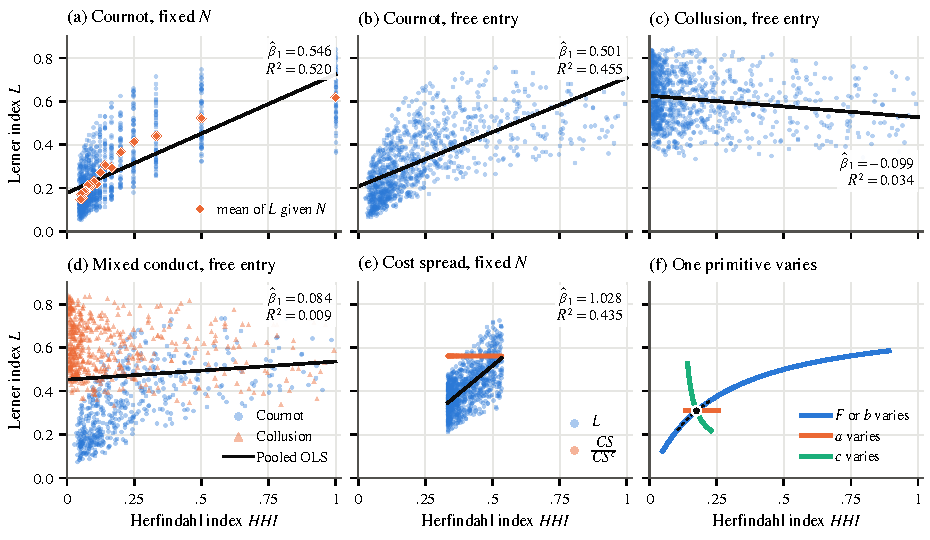
\includegraphics[width=\linewidth]{figures/ch01/scp_montecarlo.pdf}
\caption{Cross-industry SCP regressions on simulated industries. Each dot is an industry and each black
line is the OLS fit of the Lerner index on the Herfindahl index. Panel (a) also marks the mean margin at
each number of firms. Panel (d) separates Cournot and collusive industries. Panel (e) adds the consumer
surplus ratio $\frac{CS}{CS^c}$, which is the same in every industry. Panel (f) traces the free-entry
Cournot equilibrium as one primitive varies through the base point (black dot).}
\label{fig:01-montecarlo}
\end{figure}

Each of $n = 1{,}000$ industries has inverse demand $P = a - bQ$, marginal cost $c$ and fixed cost $F$.
The primitives are drawn independently, with $a \sim U[8, 12]$, $c \sim U[1, 4]$, $b \sim U[0.5, 2]$ and
$\ln F \sim U[\ln 0.1, \ln 10]$. We keep a draw only if the free-entry Cournot equilibrium has at least
one firm, which holds for 96.6 percent of draws. For each industry we compute the equilibrium
Herfindahl index and Lerner index under six designs.
\begin{enumerate}[label=(\arabic*)]
\item Cournot with a fixed number of firms $N \sim U\{1, \dots, 20\}$, drawn independently of the
primitives. Fixed costs are sunk, and in 64.4 percent of these industries the firms do not cover them.
\item Cournot with free entry, using \eqref{eq:01-fe-HL}.
\item Collusion with free entry, using \eqref{eq:01-collusion-fe}.
\item Mixed conduct with free entry, in which each industry colludes with probability $\frac{1}{2}$,
independently of its primitives.
\item Cost heterogeneity with a fixed structure. Each industry has $N = 3$ Cournot firms with marginal
costs $c_i = \bar c + \lambda (P - \bar c) z_i$, where $z = (-1, 0, 1)$ and the spread parameter
$\lambda \sim U[0, 0.95]$ is drawn independently of $(a, b, \bar c)$. The mean cost is
$\bar c \sim U[2.5, 4]$, which keeps every marginal cost positive.
\item One primitive at a time in Cournot with free entry, holding the others at the base point
$(a, c, b, F) = (10, 2.5, 1.25, 1)$.
\end{enumerate}
For designs (1) to (5) we estimate $L_k = \beta_0 + \beta_1 \HHI_k + e_k$ by OLS with
heteroskedasticity-robust standard errors in the HC1 form, which scales the White estimator by
$\frac{n}{n - 2}$. As a benchmark we compute the \emph{slope under random assignment}. It is the OLS slope of
the average causal curve $\frac{1}{n}\sum_k L_k(h)$ on $h$, with $h$ drawn from each design's own
distribution of the Herfindahl index. In designs (1), (2) and the Cournot half of (4), the causal curve of
industry $k$ is $L_k(h) = \frac{(a_k - c_k) h}{a_k h + c_k}$ (\cref{sec:01-cournot-hhi}). Under collusion it
is flat. In design (5), where concentration moves through the cost spread at fixed $N$, it is
$L_k(h) = \frac{h}{\varepsilon_k}$.
We also regress the consumer surplus ratio $\frac{CS}{CS^c}$, consumer surplus relative to its level at
price equal to (average) marginal cost, on the Herfindahl index. \Cref{fig:01-montecarlo} plots the
simulated industries and \cref{tab:01-montecarlo} reports the regressions.

\begin{table}[htbp]
\centering\small
\caption{Cross-industry OLS of the Lerner index on the Herfindahl index in 1,000 simulated industries}
\label{tab:01-montecarlo}
\begin{threeparttable}
\begin{tabular}{lccccc}
\toprule
 & \multicolumn{2}{c}{Cournot} & Collusion & Mixed & Cost spread \\
\cmidrule(lr){2-3}\cmidrule(lr){4-4}\cmidrule(lr){5-5}\cmidrule(lr){6-6}
 & Fixed $N$ & Free entry & Free entry & Free entry & Fixed $N = 3$ \\
 & (1) & (2) & (3) & (4) & (5) \\
\midrule
$\hat\beta_0$ & 0.178 & 0.208 & 0.625 & 0.453 & 0.003 \\
 & (0.004) & (0.005) & (0.005) & (0.009) & (0.016) \\
$\hat\beta_1$ & 0.546 & 0.501 & $-$0.099 & 0.084 & 1.028 \\
 & (0.022) & (0.020) & (0.016) & (0.022) & (0.042) \\
$R^2$ & 0.520 & 0.455 & 0.034 & 0.009 & 0.435 \\
Mean $\HHI$ & 0.179 & 0.238 & 0.174 & 0.206 & 0.398 \\
Mean $L$ & 0.275 & 0.327 & 0.608 & 0.470 & 0.412 \\
\midrule
Slope under random assignment & 0.535 & 0.594 & 0 & 0.340 & 1.036 \\
Slope of $\frac{CS}{CS^c}$ on $\HHI$ & $-$0.752 & $-$0.827 & 0 & $-$0.217 & 0 \\
 & (0.014) & (0.012) &  & (0.024) &  \\
\bottomrule
\end{tabular}
\begin{tablenotes}\footnotesize
\item Notes: 1,000 industries with $P = a - bQ$, marginal cost $c$ and fixed cost $F$. The primitives
$a \sim U[8, 12]$, $c \sim U[1, 4]$, $b \sim U[0.5, 2]$ and $\ln F \sim U[\ln 0.1, \ln 10]$ are drawn
independently and kept if the free-entry Cournot number of firms is at least one (96.6 percent of
draws). Column (1) draws $N \sim U\{1, \dots, 20\}$ independently of the primitives. Columns (2) to (4)
use the continuous free-entry number of firms. In column (4) each industry colludes with probability
$\frac{1}{2}$. Column (5) has 3 Cournot firms with costs $\bar c + \lambda (P - \bar c) z_i$,
$z = (-1, 0, 1)$, $\lambda \sim U[0, 0.95]$ and $\bar c \sim U[2.5, 4]$. HC1 standard errors in
parentheses. The slope under random assignment regresses the average causal curve
$\frac{1}{n}\sum_k L_k(h)$ on $h$, with $h$ drawn from the column's own distribution of $\HHI$.
$\frac{CS}{CS^c}$ is consumer surplus relative to its level at price equal to (average) marginal cost.
In columns (3) and (5) this ratio is the same in every industry, so its slope is exactly zero.
\end{tablenotes}
\end{threeparttable}
\end{table}

In design (1) the number of firms is independent of the primitives. Then $\E[L_k \mid \HHI_k = h] =
\E[L_k(h)]$, and OLS estimates the best linear approximation to the average causal curve. The estimate
$\hat\beta_1 = 0.546$ is close to the benchmark of $0.535$, and the difference is sampling error. Even here
the linear model is misspecified. Every causal curve passes through the origin and is concave
(\cref{fig:01-lerner-hhi}), and the mean margins in panel (a) trace this concavity. The fitted intercept
of $0.178$ is an artifact of fitting a line to a curve. The average derivative of the causal curves at the
observed concentrations is $1.452$, more than two and a half times the OLS slope. Most industries sit at low
concentration, where the curves are steep, while OLS gives much weight to the flat region at high
concentration.

In design (2) every industry lies on its causal curve, yet the OLS slope of $0.501$ falls about 16 percent
short of the random-assignment slope of $0.594$. The gap is the selection term of
\eqref{eq:01-potential-outcomes}. Industries become concentrated when $a - c$ is small relative to
$\sqrt{bF}$, and a small $a - c$ also lowers the causal curve $\frac{(a - c) h}{a h + c}$. The industries
observed at high concentration therefore have systematically lower curves, as in
\cref{ex:01-selection-elasticity}.

In design (3) every causal curve is flat, so concentration has no effect on margins at all. Yet OLS
reports a slope of $-0.099$ with a standard error of $0.016$. The negative sign comes from variation in
$a$ and $c$, which moves the two outcomes in opposite directions (\cref{tab:01-free-entry-cs}). Consumer
surplus is one quarter of its competitive level in every collusive industry, so concentration carries no
information about consumers either.

Design (4) mixes the two populations. The random-assignment slope is $0.340$, below the Cournot
benchmark because half of the causal curves are flat. The OLS slope is $0.084$, a quarter of the
benchmark, with an $R^2$ below one percent. Panel (d) of \cref{fig:01-montecarlo} shows why. Collusive
industries combine
high margins with low concentration and pull the pooled line toward zero.

Design (5) produces the strongest relation in the table, with $\hat\beta_1 = 1.028$ and $R^2 = 0.435$. The
benchmark slope is $1.036$, the mean of $\frac{1}{\varepsilon_k}$, because a wider cost spread raises
$L_k$ and $\HHI_k$ in the ratio $\frac{1}{\varepsilon_k}$ while leaving price unchanged. In this design the
benchmark curve comes from an intervention on the cost spread. It departs from
\cref{def:01-potential-margins}, since costs cannot stay fixed while concentration moves. In this narrower
sense the relation is causal. Yet price, output and consumer surplus are identical to those of the same industry
with symmetric costs, and $\frac{CS}{CS^c} = \frac{9}{16}$ in every industry. A researcher would see a
strong positive concentration-margin relation with no harm to consumers. \Cref{sec:01-demsetz} develops
this case.

Panel (f) isolates the comparative statics of \cref{tab:01-free-entry-cs}. Variation in $F$ or $b$ moves
the industry along an increasing concave curve, variation in $a$ moves it horizontally, and variation in
$c$ moves it down and to the right. The sign of the SCP slope depends on which primitive varies across
the sample. The slope is a property of the sample and says nothing about the technology of competition.
The fully
worked version of these models is in \cref{app:problems}.

\subsection{Panel data and fixed effects}\label{sec:01-salinger}

A natural response to omitted industry characteristics is to observe each industry several times and
remove what does not change. \citet{Salinger1990} reconsidered the concentration-margins relation with such
data. He used a Census of Manufactures panel of industries and restricted most of his analysis to
1972--84 \citep[p.~301]{Salinger1990}. Besides annual cross sections, he estimated the relation in long
differences, which remove time-invariant industry effects. The general fixed-effects version of the
regression is
\begin{equation}\label{eq:01-salinger}
\mathit{PCM}_{kt} = \alpha_k + \beta_1 \mathit{CR}_{kt} + \varphi^\top X_{kt} + e_{kt},
\qquad k = 1, \dots, n, \quad t = 1, \dots, T,
\end{equation}
where $\alpha_k$ is a fixed effect for industry $k$ and $\mathit{CR}_{kt}$ is a concentration ratio. The symbol
$\alpha_k$ is local to this subsection and differs from the price coefficient $\alpha$ of demand models. The
\emph{within estimator} subtracts each industry's time average from every variable:
\[
\mathit{PCM}_{kt} - \overline{\mathit{PCM}}_k = \beta_1 (\mathit{CR}_{kt} - \overline{\mathit{CR}}_k)
 + \varphi^\top (X_{kt} - \bar X_k) + (e_{kt} - \bar e_k),
\]
with $\overline{\mathit{PCM}}_k = \frac{1}{T}\sum_t \mathit{PCM}_{kt}$ and similarly for the other
variables. The transformation removes $\alpha_k$, and with it every time-invariant feature of the
industry, such as its demand elasticity, its technology or its accounting conventions.

With $T = 2$ the within estimator equals OLS on first differences, $\Delta \mathit{PCM}_k = \beta_1
\Delta \mathit{CR}_k + \varphi^\top \Delta X_k + \Delta e_k$. Salinger's long-difference regression has this
form without controls, plus a constant for the common change over the decade. Across 363 industries, he regressed the
change in margins from 1972 to 1982 on the change in $\mathit{CR}_4$, adjusted for market definition. The
slope is $0.178$, with a $t$-statistic of $3.49$ \citep[Table~4, row~1]{Salinger1990}. He notes that it is
roughly the size of his cross-sectional estimates \citep[p.~310]{Salinger1990}. He reads the similarity as
a sign that the cross-sectional relation could have evolved from changes in concentration over time
\citep[pp.~310--311]{Salinger1990}.

The cost is that identification now comes only from changes in concentration within an industry over
time. Consistency requires \emph{strict exogeneity}, $\E[e_{kt} \mid \mathit{CR}_{k1}, \dots,
\mathit{CR}_{kT}, X_{k1}, \dots, X_{kT}, \alpha_k] = 0$. Changes in concentration are responses to the
same demand and cost shocks that move margins. A demand boom raises margins and attracts entry, and a
cost shock can trigger exit or mergers. Such feedback violates strict exogeneity, as a simple model
shows.

\begin{example}[Entry feedback]\label{ex:01-feedback}
Let margin shocks $e_{kt}$ be independent over time with variance $\sigma_e^2$, and suppose the true
effect of concentration is $\beta_1$. Entry responds to last period's margin shock:
\[
\mathit{CR}_{kt} = \mathit{CR}_{k,t-1} - \zeta e_{k,t-1} + v_{kt}, \qquad \zeta > 0,
\]
with $v_{kt}$ independent noise of variance $\sigma_v^2$. In first differences, $\Delta \mathit{PCM}_{kt}
= \beta_1 \Delta \mathit{CR}_{kt} + \Delta e_{kt}$, where $\Delta \mathit{CR}_{kt} = -\zeta e_{k,t-1} +
v_{kt}$ and $\Delta e_{kt} = e_{kt} - e_{k,t-1}$. The two terms share $e_{k,t-1}$:
\[
\Cov(\Delta \mathit{CR}_{kt}, \Delta e_{kt}) = (-\zeta)(-\sigma_e^2) = \zeta \sigma_e^2 .
\]
With $\Var(\Delta \mathit{CR}_{kt}) = \zeta^2 \sigma_e^2 + \sigma_v^2$, the first-difference estimator
converges to
\[
\beta_1 + \frac{\zeta \sigma_e^2}{\zeta^2 \sigma_e^2 + \sigma_v^2} > \beta_1 .
\]
A favorable shock raises the margin today and attracts entry tomorrow, when the margin reverts.
Concentration and margins then fall together, and the estimator finds a positive relation even when
$\beta_1 = 0$.
\end{example}

Fixed effects also magnify measurement error. Most of the variation in concentration is between
industries and persists over time, while the within-industry changes are small. Noise in measured
concentration does not shrink in the same way. \citet{GrilichesHausman1986} make this point for panel
data in general, and the next proposition states it for the SCP regression.

\begin{proposition}[Attenuation of the within estimator]\label{prop:01-fe-attenuation}
Suppose $L_{kt} = \alpha_k + \beta_1 \HHI^*_{kt} + e_{kt}$ and we observe $\HHI_{kt} = \HHI^*_{kt} +
u_{kt}$. Industries are independent across $k$, and $T$ is fixed. The errors $u_{kt}$ are independent
across $k$ and $t$ with mean zero and variance $\sigma_u^2$, and independent of $\{\HHI^*_{ks}\}$,
$\{e_{ks}\}$ and $\alpha_k$. The shocks satisfy $\E[e_{kt} \mid \HHI^*_{k1}, \dots, \HHI^*_{kT}, \alpha_k] =
0$. Let $\sigma^2_{\tilde H} = \E\left[\frac{1}{T}\sum_t (\HHI^*_{kt} - \overline{\HHI}{}^*_k)^2\right] >
0$ be the within-industry variance of true concentration. As $n \to \infty$, the within estimator
converges to
\[
\beta_1 \, \frac{\sigma^2_{\tilde H}}{\sigma^2_{\tilde H} + \sigma^2_{\tilde u}}, \qquad
\sigma^2_{\tilde u} = \frac{T - 1}{T} \sigma_u^2 .
\]
\end{proposition}

\begin{proof}
Write $H_{kt} = \HHI_{kt}$ and $H^*_{kt} = \HHI^*_{kt}$, and write $\ddot y_{kt} = y_{kt} - \bar y_k$ for the
within transformation of any variable $y$. The fixed
effect drops out, so $\ddot L_{kt} = \beta_1 \ddot H^*_{kt} + \ddot e_{kt}$. The measured regressor
is $\ddot H_{kt} = \ddot H^*_{kt} + \ddot u_{kt}$. The within estimator is
\[
\hat\beta_1^W = \frac{\sum_k \sum_t \ddot H_{kt} \, \ddot L_{kt}}{\sum_k \sum_t \ddot H_{kt}^2}.
\]
Divide numerator and denominator by $nT$ and apply the law of large numbers across industries. The
numerator converges to
\[
\beta_1 \E\left[\frac{1}{T}\sum_t \ddot H^*_{kt} (\ddot H^*_{kt} + \ddot u_{kt})\right]
 + \E\left[\frac{1}{T}\sum_t \ddot H_{kt} \, \ddot e_{kt}\right] = \beta_1 \sigma^2_{\tilde H}.
\]
The cross term in $\ddot u_{kt}$ vanishes because $u$ is independent of $\HHI^*$. The second expectation
vanishes by strict exogeneity and the independence of $u$ and $e$. The denominator converges to
$\sigma^2_{\tilde H} + \E\left[\frac{1}{T}\sum_t \ddot u_{kt}^2\right]$. For each $t$,
\[
\E[\ddot u_{kt}^2] = \Var(u_{kt}) - 2 \Cov(u_{kt}, \bar u_k) + \Var(\bar u_k)
 = \sigma_u^2 - \frac{2\sigma_u^2}{T} + \frac{\sigma_u^2}{T} = \frac{T - 1}{T} \sigma_u^2 .
\]
Taking the ratio of the two limits gives the result.
\end{proof}

Compare the within estimator with a pooled regression that ignores the fixed effects and is valid only
if $\alpha_k$ is unrelated to concentration. Its reliability ratio is $\frac{\Var(\HHI^*)}{\Var(\HHI^*) +
\sigma_u^2}$, which uses the total variance of true concentration. The within estimator uses only the
within part. Normalize $\Var(\HHI^*) = 1$, and suppose 95 percent of it is between industries and
$\sigma_u^2 = 0.05$. The pooled reliability ratio is $\frac{1}{1.05} = 0.95$. With many periods, the
within ratio is $\frac{0.05}{0.05 + 0.05} = 0.5$, so the within estimator recovers only half of $\beta_1$.
Fixed effects remove one bias and enlarge another.

The lesson of this subsection holds for any such design. Industry fixed effects do not solve the
endogeneity of concentration, and where they remove one problem they create others: dynamic feedback
between margins and entry, and attenuation from measurement error.

\section{Efficiency, prices, and the afterlife of SCP}\label{sec:01-scp-after}

Suppose we found the econometric evidence credible: more concentrated markets have higher margins and
higher profits. Would that show that concentration is bad for consumers? This section takes up the
efficiency critique, the shift from profits to prices as the dependent variable, and the recent return of
cross-industry work in the debate over rising markups.

\subsection{Efficiency versus market power: the Demsetz critique}\label{sec:01-demsetz}

\citet{Demsetz1973} argued that concentration can be the result of superior efficiency or quality. Firms
with lower costs or better products grow, the industry becomes concentrated, and industry profits rise
because the efficient firms earn rents on their advantage. Consumers need not lose. On this view, which
became part of the Chicago critique of antitrust, the measurement may be correct while its normative
reading is wrong. \citet[p.~1013, fn.~2]{Bresnahan1989} summarizes the argument. ``Demsetz' alternative
interpretation was that high profits measure good performance, i.e.\ low costs, an argument he buttressed
by the observation that much of the profit in concentrated industries goes to large firms.'' Bresnahan
cites \citet{Demsetz1974} and notes that \citet{Bain1951} had already given a ``poor performance''
reading of the same observation. He describes the SCP literature as caught in ``a kind of gridlock'' over
whether high accounting profits signal good or bad performance \citep[p.~1013]{Bresnahan1989}.

The next proposition shows that the efficiency story holds exactly in the linear Cournot model with
heterogeneous costs.

\begin{proposition}[Concentration from cost differences]\label{prop:01-demsetz}
Let inverse demand be $P = a - bQ$, and let $N$ Cournot firms have constant marginal costs $c_1, \dots,
c_N$. Suppose all firms are active, $P > \max_i c_i$. Let $\bar c = \frac{1}{N}\sum_i c_i$ and
$\sigma_c^2 = \frac{1}{N}\sum_i (c_i - \bar c)^2$.
\begin{enumerate}[label=(\roman*)]
\item Output and price are $Q = \frac{Na - \sum_i c_i}{b(N + 1)}$ and $P = \frac{a + \sum_i c_i}{N + 1}$.
They depend on costs only through $\sum_i c_i$.
\item Shares are $s_i = \frac{P - c_i}{bQ}$, and $\HHI = \frac{1}{N} + \frac{N \sigma_c^2}{b^2 Q^2}$.
\item Industry variable profit is $\sum_i (P - c_i) q_i = bQ^2 \HHI$, and the share-weighted Lerner index
is $\sum_i s_i L_i = \frac{\HHI}{\varepsilon}$ with $\varepsilon = \frac{P}{bQ}$.
\end{enumerate}
\end{proposition}

\begin{proof}
(i) Firm $i$ maximizes $(a - bQ - c_i) q_i$. Its first-order condition is $a - bQ - b q_i - c_i = 0$, or
\[
b q_i = P - c_i .
\]
Sum over the $N$ firms: $bQ = NP - \sum_i c_i$. Substitute $P = a - bQ$:
\[
bQ = N(a - bQ) - \sum_i c_i \quad\Longrightarrow\quad bQ(N + 1) = Na - \sum_i c_i .
\]
Solve for $Q$ and substitute back into the demand curve:
\[
P = a - bQ = \frac{(N + 1)a - Na + \sum_i c_i}{N + 1} = \frac{a + \sum_i c_i}{N + 1}.
\]

(ii) The first-order condition gives $s_i = \frac{q_i}{Q} = \frac{P - c_i}{bQ}$. Because $\sum_i (P - c_i)
= bQ$, the mean of $P - c_i$ across firms is $\frac{bQ}{N} = P - \bar c$. Hence
\[
s_i - \frac{1}{N} = \frac{(P - c_i) - (P - \bar c)}{bQ} = \frac{\bar c - c_i}{bQ}.
\]
The variance of shares is $\sigma_s^2 = \frac{1}{N}\sum_i (s_i - \frac{1}{N})^2 = \frac{\sigma_c^2}{b^2
Q^2}$. By \cref{prop:01-hhi-variance}, $\HHI = \frac{1}{N} + N\sigma_s^2 = \frac{1}{N} + \frac{N
\sigma_c^2}{b^2 Q^2}$.

(iii) Using $P - c_i = b q_i$,
\[
\sum_i (P - c_i) q_i = b \sum_i q_i^2 = bQ^2 \sum_i s_i^2 = bQ^2 \HHI .
\]
Similarly, the Lerner index of firm $i$ is
\[
L_i = \frac{P - c_i}{P} = \frac{b q_i}{P} = \frac{bQ}{P} \, s_i = \frac{s_i}{\varepsilon}.
\]
Multiplying by $s_i$ and summing gives $\sum_i s_i L_i = \frac{\HHI}{\varepsilon}$.
\end{proof}

\begin{corollary}[A mean-preserving spread of costs]\label{prop:01-demsetz-spread}
Change the costs $c_i$ so that $\sum_i c_i$ is unchanged, $\sigma_c^2$ rises and all firms remain
active. Then price, output and consumer surplus $\frac{bQ^2}{2}$ are unchanged. The Herfindahl index,
industry variable profit and the share-weighted Lerner index all rise, and so does total surplus.
\end{corollary}

\begin{proof}
By \cref{prop:01-demsetz}(i), $P$ and $Q$ depend only on $\sum_i c_i$, so they and consumer surplus are
unchanged. With $Q$ fixed, part (ii) shows that $\HHI$ rises with $\sigma_c^2$. Part (iii) then shows that
industry profit $bQ^2\HHI$ and $\sum_i s_i L_i = \frac{bQ}{P}\HHI$ rise. Total surplus is consumer surplus
plus industry profit (gross of fixed costs), so it rises by the increase in profit.
\end{proof}

The corollary is the efficiency critique in one line. Across industries that differ only in the
dispersion of firm costs, concentration, margins and profits move together, and consumers are equally
well off in all of them. Design (5) of the Monte Carlo experiment is exactly this case.

\citet[Section~5.5]{Tirole1988} presents Demsetz's argument with two further examples. In Bertrand competition
with constant marginal costs, the lowest-cost firm charges the second-lowest cost and takes the whole market.
Concentration is then as high as any index that satisfies the axioms of \cref{rem:01-ej-axioms} allows, and the
firm earns a positive profit. With symmetric costs, concentration is lower and profit is zero.
\Cref{prop:01-more-draws} below studies this equilibrium when costs are random. Tirole's Exercise~5.7 is a
special case of \cref{prop:01-demsetz-spread}. Let demand be $Q = 1 - P$, so that $a = b = 1$, and let two
Cournot firms have costs $c_1 = c - d$ and $c_2 = c + d$ with $0 \le d$ and $c < 1$. The sum $c_1 + c_2 = 2c$
stays fixed as $d$ varies, and $\sigma_c^2 = d^2$. By \cref{prop:01-demsetz},
\[
  Q = \frac{2(1 - c)}{3}, \qquad P = \frac{1 + 2c}{3}, \qquad
  \HHI = \frac{1}{2} + \frac{2d^2}{Q^2} = \frac{1}{2} + \frac{9 d^2}{2(1 - c)^2} .
\]
Industry variable profit is
\[
  bQ^2 \HHI = \frac{Q^2}{2} + 2d^2 = \frac{2(1 - c)^2}{9} + 2d^2 .
\]
Both firms stay active as long as $P > c + d$, that is, $d < \frac{1 - c}{3}$. Over this range a wider cost
spread raises concentration and industry profit and leaves price unchanged.

Tirole draws a general lesson from such examples. Concentration indices give an easily computed indication of how
competitive an industry is. ``However, they have no systematic relationship with economic variables of interest
for assessing changes in cost, demand, or policy.'' With asymmetric firms, a given index need not be related in a
systematic way to welfare either. The indices are also endogenous, so their correlations with other variables
cannot be read as causal effects \citep[Section~5.5]{Tirole1988}.

The decomposition in part (ii) also shows that the source of concentration matters. Its first term,
$\frac{1}{N}$, reflects the number of firms. An extra active firm with cost $c_{N+1} < P$ lowers price,
because
\[
\frac{a + \sum_i c_i + c_{N+1}}{N + 2} < \frac{a + \sum_i c_i}{N + 1} = P
\quad\Longleftrightarrow\quad (N + 1) \, c_{N+1} < a + \sum_i c_i
\quad\Longleftrightarrow\quad c_{N+1} < P .
\]
Fewer firms therefore mean higher prices and lower consumer surplus. The second term reflects cost
dispersion, which leaves consumers unaffected. A single concentration index cannot tell the two apart.

The critique generated a large literature of firm-level \emph{horse-race regressions}. They include both
industry concentration and the firm's own market share:
\begin{equation}\label{eq:01-horse-race}
\pi_{ik} = \beta_0 + \beta_1 \mathit{CR}_k + \beta_2 s_{ik} + \varphi^\top X_{ik} + e_{ik},
\end{equation}
where $\pi_{ik}$ is the profitability of firm $i$ in industry $k$ and $s_{ik}$ its market share. The
efficiency view predicts $\beta_2 > 0$ with $\beta_1$ near zero, since large firms are profitable
because they are efficient. The market-power view predicts $\beta_1 > 0$, since concentration
facilitates high prices for all firms in the industry.

Demsetz stated the testable implication of his view himself (\citealp[p.~5]{Demsetz1973}, quoted in
\citealp[p.~46, n.~5]{LevensteinSuslow2006}). Suppose that efficiency is associated with concentration. Then
``there should be a positive correlation between concentration and the difference between the rate of return
earned by large firms and that earned by small firms.'' Let $\bar\pi^L_k$ and $\bar\pi^S_k$ be the average rates of return
of the large and the small firms in industry $k$. The implication concerns the cross-industry regression
\begin{equation}\label{eq:01-demsetz-test}
\bar\pi^L_k - \bar\pi^S_k = \gamma_0 + \gamma_1 \mathit{CR}_k + e_k ,
\end{equation}
and the efficiency view predicts $\gamma_1 > 0$. If concentration instead facilitates high prices for every firm
in the industry, the returns of small firms rise with concentration as well, and the gap need not widen. In
\eqref{eq:01-horse-race} the same contrast appears as $\beta_2 > 0$ against $\beta_1 > 0$.

Demsetz's own evidence fit the efficiency view. It was the observation, quoted above from
\citet[p.~1013, n.~2]{Bresnahan1989}, that much of the profit in concentrated industries goes to large firms.
\citet[p.~1142]{Hopenhayn1992} puts it more precisely: ``as reported by Demsetz (1973), more concentrated
industries could show higher profits for large firms and not for small ones.'' Hopenhayn also shows that the
pattern does not single out efficiency. In his competitive model of industry dynamics, a higher cost of entry
protects incumbents. It raises the profits of large firms but not necessarily those of small ones, and it raises
the market share of the largest firms. Industries with high entry costs then show the Demsetz pattern, although
every firm takes the price as given.

Later evidence was mixed. Studies that add the firm's own market share to the regression find that concentration
loses its effect \citep[Introduction, note~3]{Tirole1988}. \citet{Ravenscraft1983} reports evidence of
this kind from the line-of-business data of the Federal Trade Commission, for 3,186 business units in 258
manufacturing industries in 1975 \citep[p.~24]{Ravenscraft1983}. In the business-unit regressions of his
Table~1, the share coefficient is positive and significant. The concentration coefficient is small and negative, and significant in the generalized least squares
estimate \citep[Table~1]{Ravenscraft1983}. In the industry-level regression, which omits share, concentration has
a positive coefficient \citep[p.~26]{Ravenscraft1983}.
\citet{Schmalensee1985a} decomposed the variance of business-unit returns on assets in the 1975 line-of-business
data into industry, firm and share components. Firm effects were never statistically significant. Share effects
were significant but explained less than 1 percent of the variance. Industry effects explained about a fifth of
it, and at least 75 percent of the variance of industry average returns. About 80 percent of the variance was
unrelated to industry or share effects \citep[pp.~346--350]{Schmalensee1985a}.
Ravenscraft's paper focuses on the firm's share and Schmalensee's on the industry. Schmalensee finds the two
consistent, since share also explains less than 1 percent of the variance of profitability in Ravenscraft's
estimates \citep[p.~347]{Schmalensee1985a}. \citet[Section~5.5]{Tirole1988} and \citet[p.~46, n.~5]{LevensteinSuslow2006} point to
\citet{Schmalensee1987} for a test of collusion against differential efficiency.

The horse race cannot settle the question, because firm share is itself an equilibrium outcome. The model
of \cref{prop:01-demsetz} makes the point sharply. There, $L_{ik} = \frac{s_{ik}}{\varepsilon_k}$ for
every firm. In a sample of industries with a common elasticity $\varepsilon$, a regression of firm
margins on share and concentration returns $\beta_2 = \frac{1}{\varepsilon}$ and $\beta_1 = 0$ exactly.
Yet every firm prices above marginal cost because it internalizes the effect of its output on price,
which is market power by definition. The pattern ``$\beta_1 = 0$ and $\beta_2 > 0$'' is thus fully
consistent with a model in which firms exercise market power. It shows that margins line up with shares,
which the Cournot model of \cref{prop:01-cowling-waterson} predicts as well.

The argument has a modern echo. Dominant digital platforms attribute their large shares to the quality of
their products. Defendants have advanced this argument in recent monopolization cases. The logic is
Demsetz's: concentration may be high because some firms deliver more value per dollar, so the measured
concentration is fine and its normative reading is contested. Separating the two readings requires a
model of demand that values quality, which is the subject of \cref{ch:discrete,ch:blp}.

Efficiency and structure can also be jointly determined by competition itself. \citet{Syverson2004}
studies plants in the US ready-mixed concrete industry, where high transport costs make markets local.
Markets with denser demand have more plants, so buyers can switch between suppliers more easily. Less
efficient plants then find it harder to operate profitably, and the productivity distribution is
truncated from below. Denser markets have higher minimum and average productivity and less dispersion.
The causal arrow runs from demand density to both structure and efficiency, which no cross-industry
regression of performance on structure can capture.

\subsection{Price-concentration studies}\label{sec:01-price-concentration}

A later wave of studies replaced accounting profit with price as the dependent variable. They used
cross-sections of similar, geographically local markets within one industry
\citep[Section~3.5]{Bresnahan1989}. Examples include banking, for which \citet{Rhoades1982} lists dozens
of studies, and retail food \citep{Cotterill1986,Lamm1981}. Others cover gasoline \citep{Marvel1978},
airline city pairs \citep{GrahamKaplanSibley1983} and cement \citep{KollerWeiss1986}. \citet{Weiss1989} collected many such
studies. The estimating equation is typically a reduced form for price,
\begin{equation}\label{eq:01-price-concentration}
p_k = \beta_0 + \beta_1 \HHI_k + \varphi^\top X_k + e_k ,
\end{equation}
where $k$ now indexes local markets of one industry and $X_k$ contains demand and cost shifters. The
studies typically treat concentration as exogenous \citep[p.~1043]{Bresnahan1989}. They confirm a
positive relation between price and concentration, which is at least suggestive of market power
increasing with concentration. A variant uses changes in structure over time, as in the study of a
merger in the microfiche industry by \citet{BartonSherman1984}.

Price avoids the accounting problems of \cref{sec:01-accounting}, and similar local markets share many
omitted features. Yet the interpretation that concentration raises margins by changing conduct still
needs a defense. \citet[p.~1043]{Bresnahan1989} writes, ``I have seen no careful defense of this
interpretation, and I am troubled by it.'' He then lists difficulties which, in his words, ``have not
yet been rebutted.'' We state each one as an argument.
\begin{enumerate}[label=(\roman*)]
\item Free entry links price and concentration through scale, because larger markets fit more
firms. Take the free-entry Cournot model of \cref{sec:01-endogeneity} with $M$ consumers, so that
$b = \frac{1}{M}$. Then $P^* = c + \sqrt{\frac{F}{M}}$ and $\HHI^* = \frac{m^*}{a - c - m^*}$ with
$m^* = \sqrt{\frac{F}{M}}$, so both fall as $M$ grows. Firm output is $q^* = \frac{m^*}{b} = \sqrt{FM}$ and
average cost is $c + \frac{F}{q^*} = c + \sqrt{\frac{F}{M}} = P^*$. Firms in larger markets are larger,
have lower
average costs and break even everywhere. Price and concentration are related ``in a way that has no
obvious bad effects, and does not imply entry barriers'' \citep[p.~1044]{Bresnahan1989}.
\item Cost heterogeneity varies across markets with the same number of firms. Among such markets, the
more concentrated ones likely have more heterogeneous costs. By \cref{prop:01-demsetz}(ii),
concentration rises with $\sigma_c^2$ at fixed $N$. Cost heterogeneity may or may not interact with
conduct to raise prices.
\item Markets with more firms offer more draws on the lowest-cost firm, even if concentration is
exogenous. If that firm matters for price, price falls with the number of firms for purely
statistical reasons. \Cref{prop:01-more-draws} below formalizes the point.
\item Market-level data identify only an average of costs and conduct. Summing the first-order
conditions of \cref{prop:01-clarke-davies} with share weights gave the industry relation
\eqref{eq:01-industry-relation}. With marginal costs $mc_i$ that may vary across firms, the same steps
give Bresnahan's equation (17$'$) in our notation,
\begin{equation}\label{eq:01-avg-supply}
P = \overline{mc} - P'(Q) \, Q \, \theta, \qquad
\overline{mc} = \sum_i s_i \, mc_i, \qquad \theta = \sum_i s_i^2 (1 + r_i),
\end{equation}
which \cref{prop:01-supply-relation} derives in general. A lower price in
less concentrated markets can reflect a lower $\overline{mc}$, a lower $\theta$, or both. Most authors
have the second in mind. The two can also be linked, because a firm with a large cost advantage may
behave less competitively than it would against equal rivals.
\item The identity of the competitors matters as well as their number. \citet{GrahamKaplanSibley1983}
found that
airline city-pair markets served by carriers new to the industry have lower prices, all else equal.
These entrants very likely had
lower marginal costs, and their presence may also have changed the conditions of competition. ``Which is
it? The analysis of the paper cannot say'' \citep[p.~1044]{Bresnahan1989}. The same question applies to
the structure dummies in Porter's \citeyearpar{Porter1983} railroad cartel study.
\item Tests of the exogeneity of concentration have little power. \citet{GrahamKaplanSibley1983} tested the
exogeneity of their concentration measures and did not reject it. Their concentration coefficients
nevertheless changed
substantially when concentration was treated as endogenous. Bresnahan concludes that the test had little
power, so the assumption should not be taken as innocuous \citep[p.~1043, fn.~35]{Bresnahan1989}.
\end{enumerate}
Bresnahan stresses that these questions ``are not unanswerable'' and that the methods of
\cref{sec:01-identification} can tell marginal cost from conduct. ``The questions are, however,
unanswered'' \citep[p.~1044]{Bresnahan1989}. One clean exception he notes is \citet{SpillerFavaro1984}.
They study Uruguayan banking over a period that includes a change in entry regulation, and find that
freer entry shifts the supply relation down \citep[p.~1044, fn.~36]{Bresnahan1989}.

The more-draws argument can be made precise with order statistics, which \cref{app:math} reviews. Let
$c_{(k:N)}$ denote the $k$-th lowest of $N$ costs.

\begin{proposition}[More firms, more draws]\label{prop:01-more-draws}
Let the marginal costs of $N \ge 2$ firms be independent draws from a distribution $F_c$ on $[\underline
c, \bar c]$, and let firms compete in prices with a homogeneous good. In the equilibrium in which the
lowest-cost firm serves the market at the second-lowest cost, the price is $c_{(2:N)}$, and
\[
\E[c_{(2:N)}] = \underline c + \int_{\underline c}^{\bar c} G_N(x) \, \dd x, \qquad
G_N(x) \equiv \Pr(c_{(2:N)} > x) = (1 - F_c(x))^N + N F_c(x) (1 - F_c(x))^{N - 1}.
\]
The expected price is strictly decreasing in $N$ whenever $F_c$ is nondegenerate:
\[
\E[c_{(2:N)}] - \E[c_{(2:N+1)}] = \int_{\underline c}^{\bar c} N F_c(x)^2 (1 - F_c(x))^{N - 1} \, \dd x
> 0 .
\]
\end{proposition}

\begin{proof}
For a random variable $Y$ on $[\underline c, \bar c]$, $\E[Y] = \underline c + \int_{\underline c}^{\bar
c} \Pr(Y > x)\, \dd x$. The second-lowest cost exceeds $x$ exactly when at most one of the $N$ costs is
below $x$. No cost is below $x$ with probability $(1 - F_c(x))^N$. Exactly one is below $x$ with
probability $N F_c(x)(1 - F_c(x))^{N - 1}$. Adding the two gives $G_N(x)$. For the difference, write $F =
F_c(x)$ and compute
\begin{align*}
G_N(x) - G_{N+1}(x)
 &= (1 - F)^N \left[1 - (1 - F)\right] + F (1 - F)^{N - 1} \left[N - (N + 1)(1 - F)\right] \\
 &= F (1 - F)^N + F (1 - F)^{N - 1} \left[(N + 1)F - 1\right] \\
 &= F (1 - F)^{N - 1} \left[(1 - F) + (N + 1)F - 1\right] = N F^2 (1 - F)^{N - 1} .
\end{align*}
Integrating over $x$ gives the expression for the difference in expected prices. The integrand is
positive wherever $0 < F_c(x) < 1$, a set of positive length when $F_c$ is nondegenerate.
\end{proof}

The difference has a coupling interpretation. Adding a firm can only add a draw below $x$, so the event
``at most one cost below $x$'' becomes less likely. It fails exactly when one, and only one, of the first
$N$ costs is below $x$ and the new cost is also below $x$, which has probability
$N F_c(x)^2 (1 - F_c(x))^{N - 1}$. With costs
uniform on $[0, 1]$, $G_N(x) = (1 - x)^N + N x (1 - x)^{N - 1}$ and
\[
\E[c_{(2:N)}] = \int_0^1 (1 - x)^N \dd x + N \int_0^1 x (1 - x)^{N - 1} \dd x
 = \frac{1}{N + 1} + \frac{N}{N(N + 1)} = \frac{2}{N + 1}.
\]
The expected price is $\frac{2}{3}$ with two firms, $\frac{1}{2}$ with three and $\frac{1}{3}$ with five,
with identical Bertrand conduct in every market. In this stark model the lowest-cost firm serves the
whole market, so its share is one and the structural variable that varies is the number of firms present.
The same logic applies in any model in which the most efficient firms carry extra weight in price
determination.

\subsection{SCP today}\label{sec:01-scp-today}

SCP regressions survive as descriptive exercises. They are useful for laying out facts and empirical
regularities, such as which industries are concentrated and how margins and concentration move over
time. For the reasons in \cref{sec:01-scp-econometrics,sec:01-demsetz,sec:01-price-concentration}, they
are of little use for testing theories of market power. Schmalensee's own post-mortem concluded that the
cross-industry literature had not taught us much about how markets work
\citep[p.~160]{EinavLevin2010}.

A recent survey of health care markets restates the verdict \citep[p.~527]{HandelHo2021}. Handel and Ho note
that the SCP approach persisted longer in health economics than elsewhere. They summarize the reasons that
\citet{BerryGaynorScottMorton2019} give for the move away from it in the late 1980s. The first is measurement.
Markets are not observed directly in the data, and economic profits are hard to measure. The second is the
endogeneity of concentration. As a function of market shares, it is likely to be correlated with the unobserved
demand shifters that also move price. The third, and in their words the most fundamental, is that different
changes in primitives can produce the same correlation between concentration and prices. Mergers raise
concentration, markups and prices together and lower consumer surplus. Large firms with low marginal costs and
high fixed costs produce the same correlation, as in \citet{Demsetz1973}. So does a fall in search costs that
shifts share toward firms with high-quality products, which raises both concentration and consumer welfare
\citep{AutorEtAl2020}. The results of such regressions are therefore ``at best suggestive.'' Handel and Ho
conclude with the point of \citet{Bresnahan1989}. The effect of concentration can be studied only through three
objects: a demand system, the marginal costs of firms and the nature of oligopolistic competition.

Industry studies, the response described in \cref{sec:01-neio}, taught
much about particular industries, at the price of leaving cross-industry questions to other fields
(\cref{sec:01-today-debate}). The debate over rising markups and their role in rising inequality has
brought cross-industry, SCP-style work back, and the reactions within IO have been mixed.

\subsection{Rising markups and the production approach}\label{sec:01-rising-markups}

The recent cross-industry literature measures markups from production data instead of demand. The
approach goes back to \citet{Hall1988}, and \citet{DeLoeckerWarzynski2012} developed its firm-level
version. In this subsection $Q$ and $P$ denote the output and price of a single firm, and $\mu =
\frac{P}{mc}$ is the markup ratio of \cref{sec:01-lerner}.

\begin{proposition}[Markups from a flexible input]\label{prop:01-production-markup}
A firm produces $Q = f(V, K, \omega)$, where $V$ is a variable input bought at price $P^V$, $K$ collects
the other inputs and $\omega$ is productivity. Suppose the firm minimizes cost, takes $P^V$ as given,
and adjusts $V$ freely. Let $\lambda$ be the multiplier on the output constraint. Then $\lambda = mc$ and
\[
\mu = \frac{P}{\lambda} = \phi^V \frac{PQ}{P^V V}, \qquad
\phi^V = \frac{\partial f}{\partial V} \frac{V}{Q},
\]
where $\phi^V$ is the output elasticity of the variable input.
\end{proposition}

\begin{proof}
The firm chooses $V$ to minimize $P^V V$ plus the cost of the other inputs subject to $f(V, K, \omega) \ge
Q$. The Lagrangian is
\[
\mathcal{L} = P^V V + C^K(K) - \lambda \left[ f(V, K, \omega) - Q \right],
\]
where $C^K(K)$ is the cost of the other inputs. The first-order condition for $V$ is
\[
P^V = \lambda \frac{\partial f}{\partial V}.
\]
By the envelope theorem (\cref{app:math}), the derivative of minimized cost with respect to $Q$ equals
$\frac{\partial \mathcal{L}}{\partial Q} = \lambda$, so $\lambda = mc$. Multiply the first-order condition
by $\frac{V}{\lambda Q}$:
\[
\frac{P^V V}{\lambda Q} = \frac{\partial f}{\partial V} \frac{V}{Q} = \phi^V .
\]
Solve for $\lambda = \frac{P^V V}{\phi^V Q}$ and divide price by it:
\[
\mu = \frac{P}{\lambda} = \frac{P \phi^V Q}{P^V V} = \phi^V \frac{PQ}{P^V V}.
\qedhere
\]
\end{proof}

The formula needs no demand model and no assumption about conduct. The markup is the output elasticity
of a flexible input divided by that input's share of revenue. Its appeal for cross-industry work is
obvious, because revenue shares are available in accounting data for many firms.

\citet{DeLoeckerEeckhoutUnger2020} applied the formula to US publicly listed firms in the Compustat data from
1955 to 2016, treating cost of goods sold as the variable input. Each firm's markup is the ratio of its revenue
to its cost of goods sold, multiplied by an estimated output elasticity of the variable inputs. The method
follows \citet{DeLoeckerWarzynski2012}, and the firm markups are then averaged with revenue weights
\citep[p.~258 and n.~203]{AskerNocke2021}. As read from the figure in \citet[Figure~11, p.~259]{AskerNocke2021},
the revenue-weighted average markup rose from about 1.21 in 1980 to about 1.61 in 2016. The rise was confined to
the upper tail. The median markup is flat over the period, and in the authors' own words, ``Most firms see no
increase in markups. For the higher percentiles, markups increase. For the 90th percentile in particular, the
increase is sharpest. Between 1980 and 2016, it increases from 1.5 to 2.5'' (quoted in
\citealp[p.~258]{AskerNocke2021}). The rise in the average is thus ``largely driven by a few firms that currently
have much higher markups than decades ago.'' The finding drew wide attention because it suggested a rise in
market power across the economy. \citet{DeLoeckerSyverson2021} survey the production approach behind it, and
their chapter closes with its use to measure market power in product and labor markets
\citep[Preface, p.~xvi]{HoHortacsuLizzeri2021}.

The critiques mirror the problems of the SCP literature.
\begin{itemize}
\item The output elasticity $\phi^V$ must be estimated, usually from a production function by industry.
Most data record revenue instead of physical output. With revenue $R = PQ$ and profit maximization,
which sets marginal revenue $MR$ equal to $mc = \lambda$, the elasticity of revenue with respect to $V$ is
\[
\frac{\partial \ln R}{\partial \ln V} = \frac{\partial \ln R}{\partial \ln Q} \, \phi^V
 = \frac{MR}{P} \, \phi^V = \frac{\phi^V}{\mu}.
\]
Plugging this revenue elasticity into \cref{prop:01-production-markup} in place of $\phi^V$ gives
\[
\frac{\phi^V}{\mu} \cdot \frac{PQ}{P^V V} = \frac{\mu}{\mu} = 1
\]
for every firm. A revenue elasticity therefore carries no information about the markup, a point
developed by \citet{BondEtAl2021}.
\item A markup ratio above one must cover fixed and overhead costs (\cref{prop:01-zero-profit-markup}).
If technology has shifted toward fixed costs, such as software and overhead, $\mu$ rises with no rise in
profits. Which costs count as variable, cost of goods sold or also overhead, matters for the trend. A shift
of the population toward firms with larger fixed costs or lower costs of goods sold moves the average markup
by composition alone \citep[p.~258]{AskerNocke2021}. De Loecker, Eeckhout and Unger reply that the rise in
markups ``is not merely to offset a rise in overhead costs'' (quoted in \citealp[p.~258, n.~205]{AskerNocke2021}).
They find that markups rose by more than overhead costs, and that the excess markups are highest for the firms
with high overhead costs. Their measure of profits rose too, as did market value as a share of sales.
\item The average depends on the weights. A revenue-weighted mean rises when sales move toward large firms
with high markups, even if no firm's markup changes.
\item The relation between markups and concentration across industries is subject to every problem of
\cref{sec:01-scp-econometrics}.
\end{itemize}
Descriptive evidence on concentration itself gives a modern version of the Demsetz pattern of
\cref{sec:01-demsetz}. \citet{Ganapati2020} examines detailed firm-level Census data for 1972--2012. As reported
by \citet[p.~259]{AskerNocke2021}, increases in concentration are positively correlated with productivity and with real output growth. They are
uncorrelated with price changes and with overall payroll, and they are negatively correlated with labor's share
of revenue. Concentration rose where output and productivity grew, without the price increases that the
market-power reading would predict. This fits the efficiency reading better than the market-power reading,
although, as \cref{sec:01-demsetz} showed, it cannot rule out market power.

\citet{BerryGaynorScottMorton2019}, to whom \citet[p.~259, n.~206]{AskerNocke2021} point for an IO perspective on
this literature, develop the last point of the bulleted list above.
Their argument, summarized in \cref{sec:01-scp-today}, is that different changes in primitives can produce the
same correlation between concentration and markups, with very different positive and normative implications
\citep[p.~47]{BerryGaynorScottMorton2019}.
Following \citet{Bresnahan1989}, they hold that the effect of concentration cannot be interpreted without
demand, the marginal costs of firms and the nature of oligopolistic competition
\citep[p.~48]{BerryGaynorScottMorton2019}. They regard the production
approach as persuasive evidence that markups have risen, although the size and causes of the rise remain open
\citep[p.~49]{BerryGaynorScottMorton2019}.
Because industries are so heterogeneous, they argue that careful industry studies are also needed. They call
for many more such studies \citep[pp.~50 and 53]{BerryGaynorScottMorton2019}.

A demand-side study of one large industry models these three objects and reaches a contrasting answer.

\casehead{The US automobile industry}\citet{GriecoMurryYurukoglu2024}, GMY below, ask whether market power in the
US new-car market rose between 1980 and 2018, a period over which the production approach reports rising markups. We cite
the author manuscript on hand, whose title page is dated July 5, 2023. Its table and figure numbers may differ
from those of the published article.
Product data from Ward's Automotive give the sales, list prices and characteristics of new
cars and light trucks. An observation is a make-model-year, such as the 1987 Honda Accord, and the sample has
9,694 of them (Table~I). The market size is the number of US households divided by 2.5. The divisor reflects that
a household owns nearly two cars and keeps each for about five years. Survey data add the demographics of buyers
and the models they name as their second choices.

\casehead{Model and identification}Demand is a random coefficients logit of the kind developed in \cref{ch:blp}.
Household $i$ in year $t$ obtains from model $j$ the utility
\[
  u_{ijt} = x_{jt}\beta_i - \alpha_i p_{jt} + \xi_{jt} + \epsilon_{ijt}
\]
in our sign convention for price (their equation 1). The tastes $(\alpha_i, \beta_i)$ depend on demographics drawn
from the Current Population Survey and on normal taste shocks (equations 3 and 4). Manufacturers set the prices of
all their models in a static Nash-Bertrand game each year. The first-order conditions are those of
\cref{prop:01-multiproduct-foc} (their equation 6). GMY solve them for the marginal cost of every model at the
estimated demand parameters, as in \eqref{eq:01-implied-mc}. The price instrument is the real exchange rate of the
country where the model is built, lagged one year and taken from the Penn World Table. It moves with local labor
costs and with the nominal exchange rate, so it shifts the cost of supplying the US market. Average unobserved
quality and the value of the outside good both move the total share of new cars each year. The year effects alone
cannot separate them. GMY follow \citet{PakesBerryLevinsohn1993} and assume that, for models sold in two
consecutive years without a redesign, the change in $\xi_{jt}$ has mean zero (their equation 2).

Estimation is by the generalized method of moments (GMM) in three steps (their Section~5). The first matches micro moments, such as the average price paid
by each income quintile and the correlation of characteristics between first and second choices. The second
regresses the estimated mean utilities on characteristics, price, make and year dummies by two-stage least
squares with the exchange-rate instrument. The third applies the continuing-model restriction to the estimated
year effects. Standard errors come from a bootstrap of the micro data.

\begin{table}[htbp]
\centering
\caption{Markups, concentration and welfare in the US new-car market}
\label{tab:01-gmy}
\small
\begin{tabular}{@{}lrrl@{}}
\toprule
\multicolumn{4}{@{}l}{\textit{Panel A. Baseline estimates}} \\
\addlinespace[2pt]
 & 1980 & 2018 & Source \\
\midrule
Median Lerner index & 0.325 & 0.185 & Figure VIa, p.~2 \\
Share-weighted mean Lerner index & 0.42 & 0.22 & Table VII \\
Share-weighted mean Lerner index, log price & 0.32 & 0.27 & p.~21 \\
Herfindahl index (HHI points) & 2661 & 1132 & Table VII \\
Consumers' share of total surplus & 0.62 & 0.82 & p.~2 \\
\bottomrule
\end{tabular}

\medskip
\begin{tabular}{@{}lrr@{}}
\toprule
\multicolumn{3}{@{}l}{\textit{Panel B. Hypothetical cartels in 2018 (Table VII)}} \\
\addlinespace[2pt]
Cartel members & Mean Lerner index & HHI points \\
\midrule
None (2018 baseline) & 0.22 & 1132 \\
GM, Ford and Toyota & 0.26 & 2546 \\
Top three and Fiat & 0.35 & 3724 \\
Top four and Honda & 0.39 & 4819 \\
Top five and Nissan & 0.46 & 6000 \\
\bottomrule
\end{tabular}
\par\smallskip
\begin{minipage}{\textwidth}\footnotesize
\textit{Notes:} The Lerner index is $\frac{p - mc}{p}$, with marginal costs implied by Nash-Bertrand pricing.
Means are weighted by market shares. Total surplus is the sum of consumer surplus, producer surplus and deadweight
loss, which the authors call efficient surplus. In Panel B, parent companies join the cartel in order of 2018
sales, and Fiat is the parent of Chrysler. Source: Grieco, Murry and Yurukoglu (2024), author manuscript (title
page dated July 5, 2023), with the table, figure and page numbers of that manuscript.
\end{minipage}
\end{table}

\casehead{Results}\Cref{tab:01-gmy} collects the main numbers. The median Lerner index fell from 0.325 in 1980 to
0.185 in 2018, and the share-weighted mean fell from 0.42 to 0.22 (Figure~VIa and Table~VII). Markups fell across
the distribution, for every vehicle style and for imported as well as domestic models (Figures~VI and~VII). Demand
became more elastic. The share-weighted average own-price elasticity was $-4.23$ in 1985 and $-5.36$ in 2015, and
the market elasticity moved from $-1.07$ to $-1.29$ (Table~V). Concentration fell as well, and consumers gained.
The share of total surplus going to consumers rose from 0.62 to 0.82, and consumer surplus per household rose by
roughly \$8,000 (p.~2). GMY attribute the gain mainly to better product quality and better production technology.

Two checks address the main threats to this conclusion. With log price in utility in place of price, the mean
Lerner index still falls, from 0.32 to 0.27 (p.~21). The supply side assumes Nash-Bertrand pricing throughout, so
a move toward collusion could hide rising market power. Under fixed alternative conduct, collusion among the three
US manufacturers or among all firms, markups still decline (Figure~X). Panel~B of \cref{tab:01-gmy} asks how large
a cartel in 2018 would have to be to restore the 1980 mean of 0.42. Only a cartel of the six largest parent
companies exceeds it. GMY judge that a cartel of that scale would hardly escape the notice of antitrust
authorities (p.~27).

\casehead{Comparison with the production approach}GMY compare their series with the auto-industry estimates
of \citet{DeLoeckerEeckhoutUnger2020} in their Section~5.6 and Figure~XI. They also restate the
economy-wide rise from 1.21 to 1.61 in the sales-weighted ratio of price to marginal cost (p.~28), which matches
the figures above. The two auto series differ in level and in trend, although both are fairly flat after 1995. GMY
give three reasons why the production approach may fail in this industry. First, cost of goods sold includes fixed
manufacturing overhead under US accounting rules, so it is not the freely chosen input that
\cref{prop:01-production-markup} requires. Second, the output elasticity is estimated from revenue in place of
physical output, as in the critique of \citet{BondEtAl2021}. It is also pooled with firms in many other
manufacturing industries that share its two-digit code. Third, Compustat covers only listed firms. Several
manufacturers that sell in the US never appear in it, and its revenues include sales outside the US and of other
products.

The next example shows why a markup, even a correctly measured one, is a poor guide to welfare when products
improve.

\begin{example}[Quality, markups and consumer surplus]\label{ex:01-quality-markup}
This example follows \citet[p.~26, n.~13]{GriecoMurryYurukoglu2024}. A monopolist sells one product with constant
marginal cost $mc$ to $M$ consumers, who may instead choose an outside good. Consumer $i$ obtains utility
$\xi - \alpha p + \epsilon_{i}$ from the product and $\epsilon_{i0}$ from the outside good. The shocks are type-I
extreme value, and $\xi$ measures quality. Let $v = \xi - \alpha p$. The share of buyers and its price derivative
are
\[
  s = \frac{e^{v}}{1 + e^{v}}, \qquad \frac{\partial s}{\partial p} = -\alpha s (1 - s).
\]
The first-order condition $s + (p - mc)\frac{\partial s}{\partial p} = 0$ gives the dollar markup
\[
  p - mc = \frac{1}{\alpha (1 - s)} .
\]
Now raise quality and hold $mc$ fixed. Since $\dd s = s(1 - s)\,\dd v$ and $\dd v = \dd\xi - \alpha\,\dd p$,
differentiating the markup equation gives
\[
  \dd p = \frac{\dd s}{\alpha (1 - s)^2} = \frac{s}{\alpha (1 - s)}\left(\dd\xi - \alpha\,\dd p\right).
\]
Collect the terms in $\dd p$, using $1 + \frac{s}{1 - s} = \frac{1}{1 - s}$:
\[
  \frac{\dd p}{1 - s} = \frac{s}{\alpha (1 - s)}\,\dd\xi
  \quad\Longrightarrow\quad
  \frac{\dd p}{\dd \xi} = \frac{s}{\alpha} > 0 .
\]
The dollar markup rises one for one with price. The Lerner index rises too, because
\[
  \frac{\dd}{\dd \xi}\left(\frac{p - mc}{p}\right) = \frac{mc}{p^2}\,\frac{\dd p}{\dd \xi} > 0 .
\]
Yet the net utility of the product rises as well:
\[
  \frac{\dd v}{\dd \xi} = 1 - \alpha\,\frac{\dd p}{\dd \xi} = 1 - s > 0 .
\]
Consumer surplus is $\frac{M}{\alpha}\ln(1 + e^{v})$ up to a constant, by the log-sum formula of
\cref{sec:07-logsum}, so it rises with $v$. A better product raises the markup, by either measure, and consumer
surplus at the same time.
\end{example}

The data of GMY show the converse case. Better cars were also costlier to build. Over 1980 to 1999, average shares
and their price derivatives were stable while average prices rose (their Section~5.4.1 and Figure~VIII). For a
single-product firm the first-order condition gives
\[
  \frac{p - mc}{p} = -\frac{1}{p}\, s \left(\frac{\partial s}{\partial p}\right)^{-1}
\]
(their equation 7). Stable shares and derivatives keep the dollar margin fixed, so a higher price lowers the Lerner
index. A counterfactual that holds observed characteristics at their 1980 distribution removes the rise in
marginal cost and much of the fall in markups (Figure~IX). In both directions the lesson is the one GMY draw. A
markup is a poor measure of performance over long periods in which products change (p.~2). \Cref{ch:blp} develops
the model behind such studies, and \cref{app:problems} estimates simpler demand models on the replication data of
GMY.

The SCP paradigm and its critics leave one lesson for the rest of the book. Cross-industry correlations
between margins and concentration cannot separate demand, cost and conduct, because all three determine
both variables at once. The response is to study one industry at a time, with a model of its demand,
its costs and the conduct of its firms. \Cref{sec:01-neio} turns to that response.
